%!TEX root = main.tex
\section{Precise Visual Querying\label{sec:precise}}
While visual analysis often reveal important anomalies or trends in the data~\cite{Heer2012,Morton2014}, it is often challenging to choose the right piece of data to visualize in order to realize these insights. In this section, we first motivate the use case for visual query systems and describe \zv as an example of such a system built to address these challenges.
\subsection{Motivating Example}
Astronomers from the the Dark Energy Survey (DES) are interested in finding anomalous time series to discover astrophysical transients (objects whose brightness changes dramatically as a function of time), such as supernova explosions or quasars~\cite{Drlica-Wagner2017}. When trying to find celestial objects corresponding to supernovae, which have a specific pattern of brightness over time, scientists need to individually inspect the visualizations of each object until they find ones that match the pattern. With more than 400 million objects in their catalog, each having their own set of time series brightness measurement, the process of manually exploring a large number of visualizations is not only error-prone, but also overwhelming for scientists who do not have extensive knowledge about their dataset.  
% Intention driven task-based querying (Precise search)
\par The astronomy use case highlights a common challenge in exploratory data analysis (EDA). There is often a large space of possible visualizations that could be generated from a given dataset and manual search through this large collection is inefficient. Popular visualization authoring tools such as Tableau and Excel focus on presenting one visualization at a time and there is no systematic way to create, compare, and query large collections of visualizations. 
%\par There has been many related work in this space varying different dimensions of possible visualizations, including visual encodings~\cite{showme}, data facets, . We will focus on  
\subsection{Effortless Data Exploration with \zv}
\par The challenges discussed in the previous section point to the need for a tool that enables users to create and search through large collections of visualizations. To this end, we developed \zv, a \emph{precise visual querying system (PVQS)} that accepts precise queries in the form of a desired pattern specified through frontend interactions and returns a ranked list of visualizations that look similar to the input pattern~\cite{Siddiqui2016}. \zv is built on top of a querying language called ZQL, which provides a mechanism for managing collections of visualizations. Contrary to prior work on visualization languages for specifying visual encodings of individual visualizations~\cite{Stolte2002,Wilkinson2005}, ZQL supports high-level queries over visualization collections, such as composing, sorting, filtering a collection of visualization. ZQL functionals and primitives can be constructed into rich and expressive query semantics, with functionalties including: 
\begin{itemize}
	\item Finding top-k visualizations whose y values are most or least similar from a queried visualization. (e.g. Find cities with sold price over time similar to Manhattan. Varying along \textsc{city} while keeping \textsc{x = time,y = AVG(price)} fixed.) 
	\item Comparing across a collection of visualizations by iterating over one or more x, y, z attributes while fixing other attributes. (e.g. Find an y attribute that varies with time similarly how average price changes over time)
	\item Finding a pair of X and Y axes where two specific visualization instances differ the most. (e.g. Finding pairs of attributes where visualizations for the products `stapler' and `chair' differ the most.)
\end{itemize}
\par Given a ZQL query, \zv parses the query into a graph of visual component nodes (containing visualization information, such as X, Y columns) and task nodes (common and user-defined primitives for processing visual components, such as sort or filter). \zv then performs query optimization to merge together multiple nodes, as well as reducing the processing time required for individual visualization components. Using the optimized query plan, the executor compiles visual nodes into SQL queries for retrieving the visualization data and postprocesses the result via the defined operations. 
\par While ZQL provides powerful mechanism for expressively specifying queries on large collections visualizations, writing ZQL queries can be daunting for novice users. Therefore, we extracted a typical workflow of visualization querying (finding top-k most similar visualization from a collection with fixed X,Y while varying Z) to allow users to formulate ZQL queries through interactions. The user can either perform frontend interactions mapped onto ZQL queries or directly input ZQL queries through a table input. The query results are rendered as a ranked list of visualizations in the results panel in the interface. \zv is a full-fledged visual querying system that supports a variety of querying interactions as illustrated in Figure~\ref{fig:modalities}. In the following section, we will discuss the design process of the interactions in this precise visual query system and the lessons that we have learned for designing future visual data exploration systems.

\begin{figure}[h!]
\centering
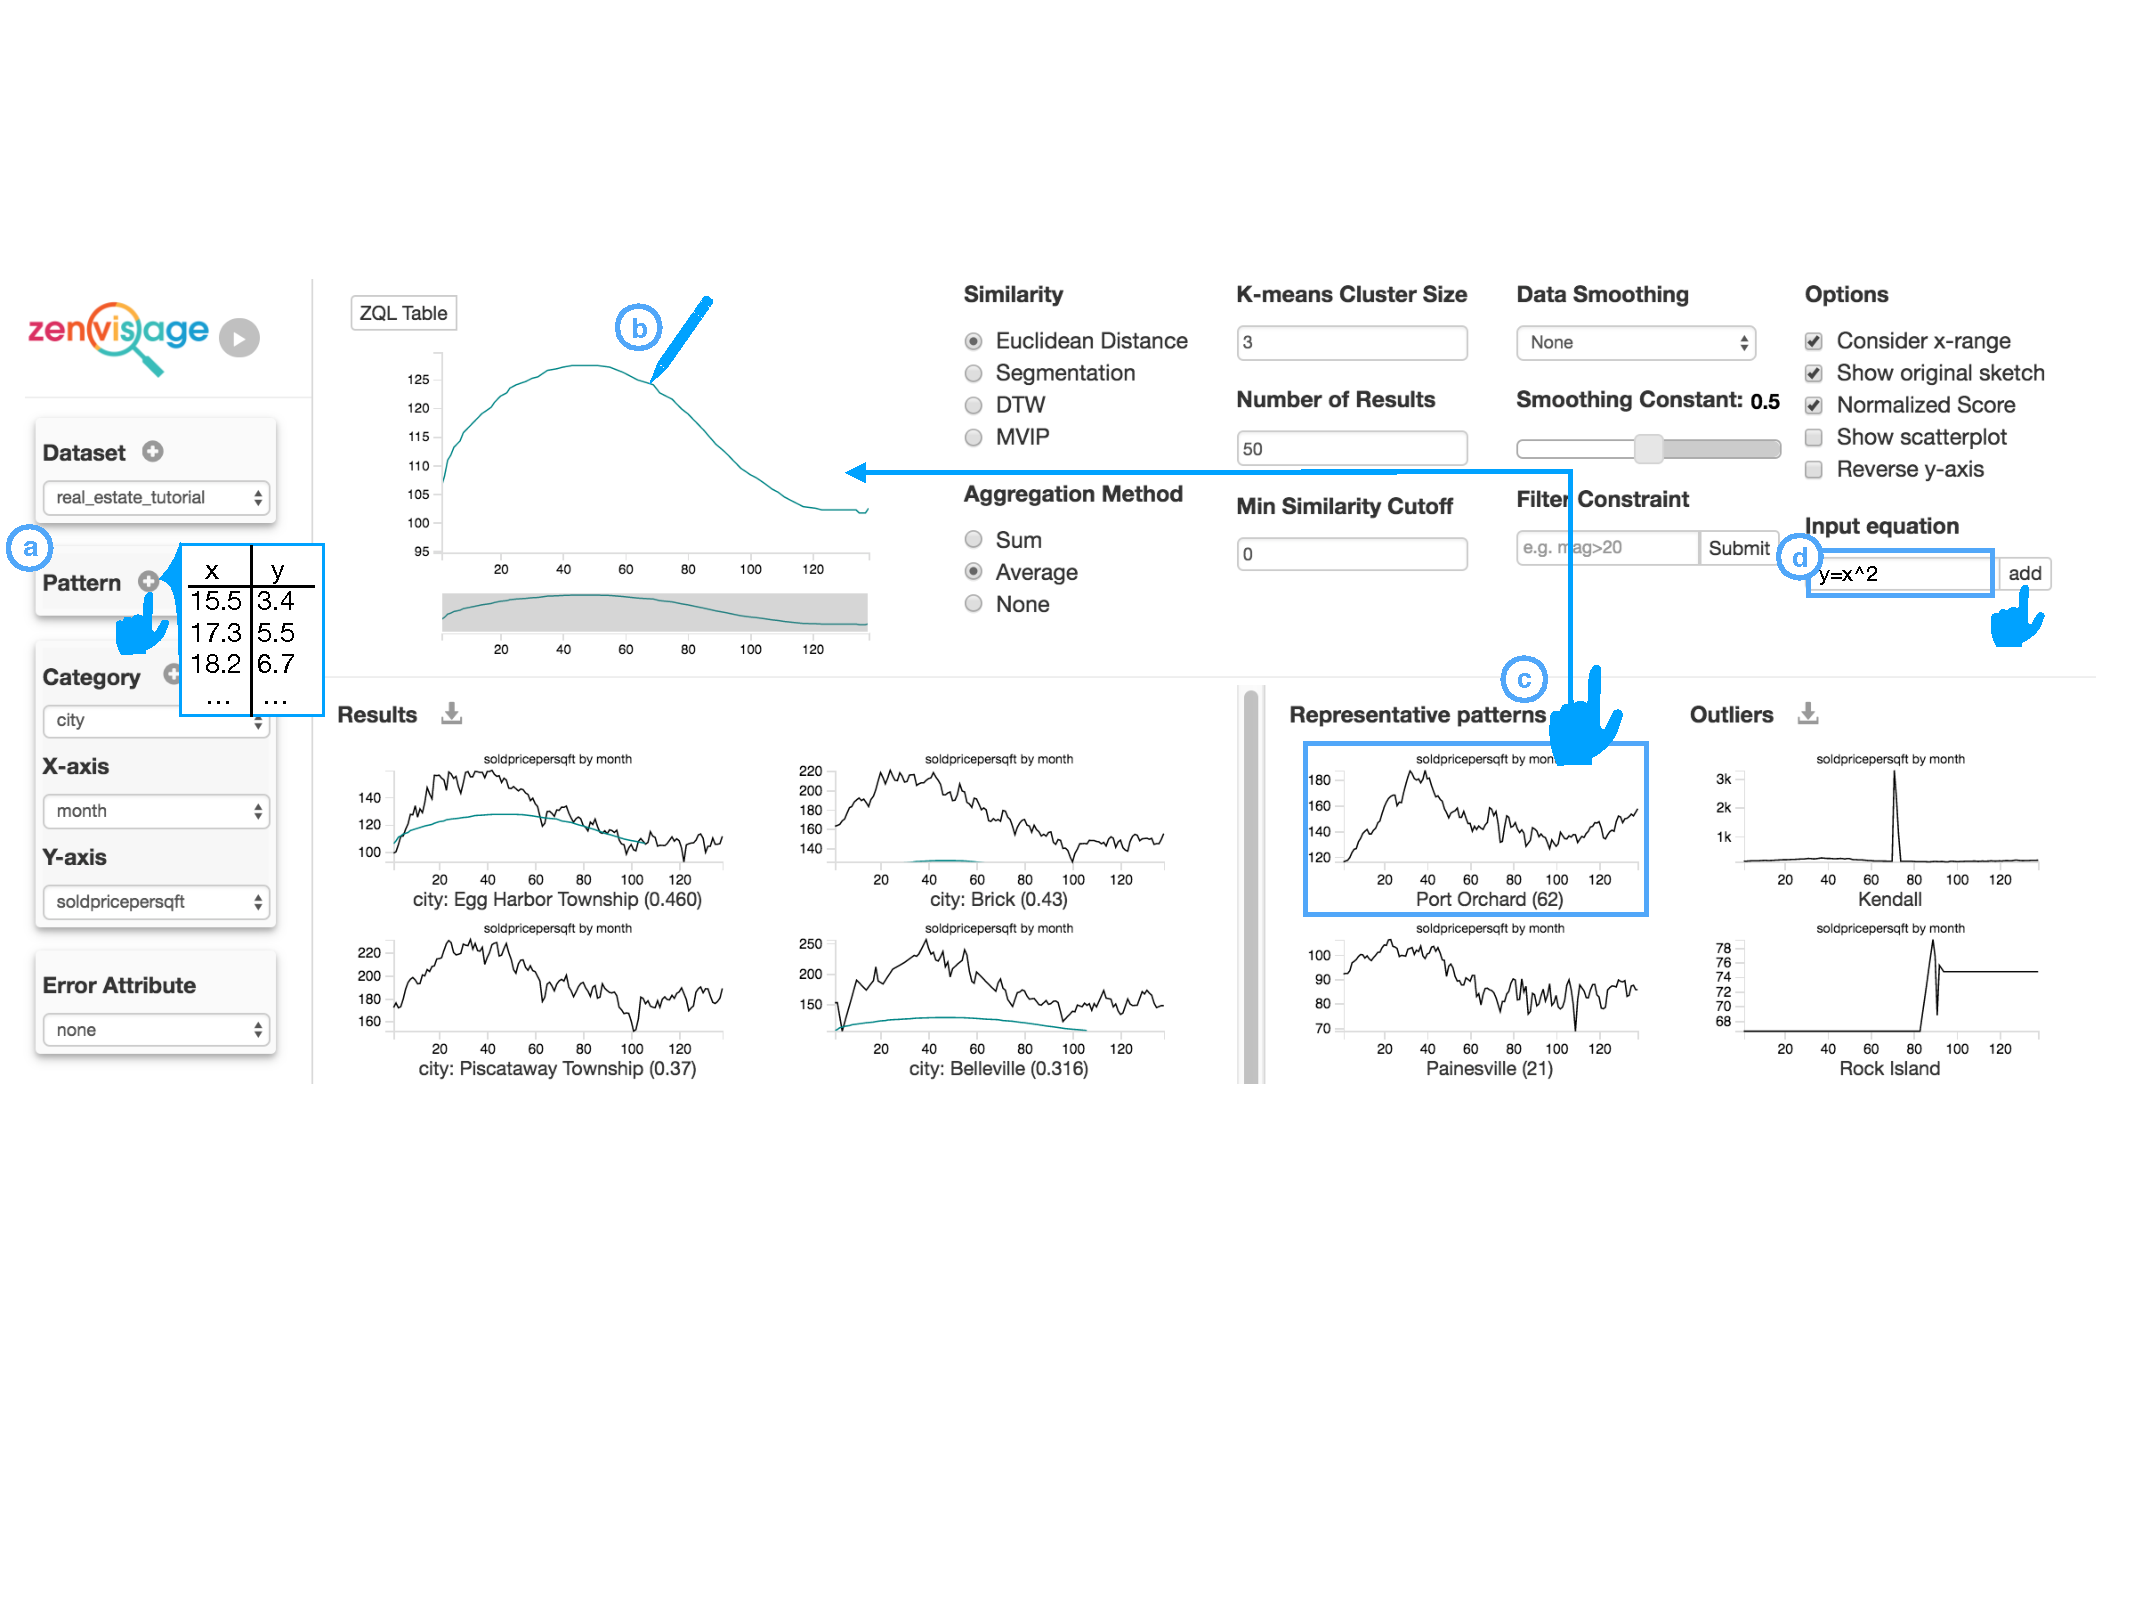
\includegraphics[width=0.8\textwidth]{figures/modalities.pdf}
\caption{\zv offers a variety of querying modalities, including: a) uploading a sample pattern from an external dataset as a query, b) sketching a query pattern, c) dragging-and-dropping an existing pattern from the dataset, and d) inputting an equation as a query, from \cite{Lee2017}.}
\label{fig:modalities}
\end{figure}
\subsection{Challenges of Precise Visual Querying Systems}
\par In developing \zv, we collaborated with scientists from astronomy, genetics, and material science in a year-long participatory design process~\cite{Lee2017}. In particular, we studied how various features impact analysts' ability to rapidly generate new hypotheses and insights and perform visual querying and analysis. We employed Pirolli and Card's information foraging theory to contextualize our study results~\cite{Pirolli}. Our findings not only offers design guidelines for improving the usability and adoption of next-generation PVQSs, but more importantly, points towards the need for supporting other components in the cycle of visual data exploration. %can be 

\stitle{The Problem of Ambiguous, High-level Queries}
%\subsection{The Need for Visual Querying Expressivity}%Supporting Vague and Complex Querying
\par When users query with a PVQS, they often translate their ambiguous, high-level questions into an plan that consists of multiple interactions to incrementally address their desired query. %Participants in our \zv design study often created unexpected workflows that chained together analysis steps consisting of multiple interactions and controls. For example, geneticists in our study repeatedly explored representative trends to gain an overall sense of the typical profiles that exist in their dataset and queried mainly through drag-and-drop of these representative trends. Variations to their main workflow also include changing cluster sizes and display control settings to offer them different perspectives on the dataset. 
The expressiveness of PVQSs comes from the multiplicative effect of stringing together combinations of interaction sequences into a customized workflow. Designing features that diversifies potential variations expands the space of possible workflows that could be constructed during the analysis. However, even with many supported interactions, there were still vague and complex queries that could not be decomposed into a multi-step interaction workflow. For example, \zv was unable to support high-level queries that involved the use of vague descriptors for matching to specific data characteristics, such as finding light curves that are flat and `without noise', or patterns that `exhibits irregularities'. %While this could be expressed through user-defined functions in the underlying querying language ZQL, the learning curve and engineering cost is high. %Our previous example of queries that could not be expressed in the \zv interface showcases one example of  %\dor{Not sure if its worthwhile to include a couple sentences about Tarique's regex/NLP work here. e.g. the `up and then down' example}. 
These scenarios showcase examples of lexical ambiguity, where the PVQS can not map the vague term `irregular' or `noisy' into the appropriate series of analysis steps required to find these patterns. In Section~\ref{sec:vague}, we survey the challenges of PVQSs in supporting vague and complex queries and point to several promising directions of ongoing research in this area.

\stitle{The Problem of Not Knowing What to Query}
\par Another key design principle that came from this study was the need for visualization recommendations that can help analysts jump-start their exploration. For example, we found that many users made use of the recommended representative trends and outliers visualizations provided by \zv as contextual information to better understand their data or to query based on these recommended visualizations. In addition, they often query using these recommended visualizations in a bottom-up approach, rather than coming up with a query in a top-down, prescriptive manner.  This behaviour explained by the fact that participants often start their analysis with a pattern in mind, without knowing what the data looks like, so don't know what to query for. Recommendations facilitate a smoother flow of analysis by closing the loop between the two modalities of querying and exploration, reminiscent of the browsing and searching behaviors on the Web~\cite{Olston2003}, thus ensuring that user is never stuck or out of ideas at any point during the analysis. Typically, visualization recommendation system seeks to accelerate the process of discovering interesting aspects of the data by broadening exploration. In Section~\ref{sec:understanding}, we advocate that recommendation systems should not only focus on data discoverability aspect of exploration, but also contribute towards helping users become more aware of the distributions in their data and the context of their analysis.
% % \subsection{Top-down and Bottom-up Querying Modalities}
% % \par Our study also revealed the challenges of coming up with a query in a prescriptive manner. 
% % Need a topic sentence/paragraph
% \par Pirolli and Card's notional model distinguishes between information processing tasks that are \textit{top-down} (from theory to data) and \textit{bottom-up} (from data to theory)~\cite{Pirolli}. In the context of visual querying, users employ top-down approaches by starting with a hypothesis on what patterns to look for and express it through sketching or inputting an equation (Figure~\ref{fig:modalities}b,d). On the other hand, bottom-up approaches originate from the data (or equivalently, the visualization). For example, the user may drag and drop a visualization of interest in the dataset as the input query or upload a visualization from an external dataset (Figure~\ref{fig:modalities}a,c). These two modalities of querying are reminiscent of the browsing and searching behaviors on the Web, which derives from the successful application of foraging theory to Web Search~\cite{Olston2003}.
% \par While the usage of each querying feature may vary from one participant to the next, our interactions with the scientists showed that \emph{bottom-up querying via drag-and-drop was more intuitive and more commonly used than top-down querying methods when the users have no desired patterns in mind}, which is commonly the case for exploratory data analysis. One of the main reason why participants did not find sketching useful was that they often do not start their analysis with a pattern in mind. Later, their intuition about what to query is derived from other visualizations that they see in the PVQS, in which case it made more sense to query using those visualizations as examples directly. Similarly, while functional fitting is a common operation in scientific data analysis, querying by equation is also unpopular, since it is challenging to formulate functional forms in an prescriptive, ad-hoc manner without seeing what the common patterns in the dataset are. 
%  %(e.g. after a filter is applied)  (e.g. find visualizations that are similar to the one in the largest representative clusters). 
% \par As evident from the representative and outliers visualization recommendations in \zv, recommendations facilitate a smoother flow of analysis by closing the loop between the two modalities of querying and exploration, thus ensuring that user is never stuck or out of ideas at any point during the analysis. Typically, visualization recommendation systems seeks to accelerate the process of discovering interesting aspects of the data by broadening exploration. In Section~\ref{sec:understanding}, we advocate recommendation systems should not only focus on data discoverability aspect of exploration, but also contribute towards helping users become more aware of the distributions in their data and the context of their analysis.